\documentclass[11pt,letterpaper]{article}

\addtolength{\oddsidemargin}{-.875in}
\addtolength{\evensidemargin}{-.875in}
\addtolength{\textwidth}{1.75in}

\addtolength{\topmargin}{-.875in}
\addtolength{\textheight}{1.75in}

\usepackage[utf8]{inputenc}
\usepackage{caption} % for table captions
\usepackage{amsmath} % for multi-line equations and piecewises
\DeclareMathOperator{\sign}{sign}
\usepackage{graphicx}
\usepackage{relsize}
\usepackage{xspace}
\usepackage{verbatim} % for block comments
\usepackage{subcaption} % for subfigures
\usepackage{enumitem} % for a) b) c) lists
\newcommand{\Cyclus}{\textsc{Cyclus}\xspace}%
\newcommand{\Cycamore}{\textsc{Cycamore}\xspace}%
\newcommand{\deploy}{\texttt{d3ploy}\xspace}%
\newcommand{\Deploy}{\texttt{D3ploy}\xspace}%
\usepackage{tabularx}
\usepackage{color}
\usepackage{multirow}
\usepackage{float} 
\usepackage[acronym,toc]{glossaries}
%\newacronym{ANL}{ANL}{Argonne National Laboratory}
\newacronym{B4C}{B4C}{boron carbide}
\newacronym{BC}{BC}{boundary condition}
\newacronym{BOC}{BOC}{beginning of equilibrium cycle}
\newacronym{BSD}{BSD}{Berkeley Software Distribution}
\newacronym{BWR}{BWR}{Boiling Water Reactor}
\newacronym{CAISO}{CAISO}{California ISO}
\newacronym{CEA}{CEA}{Commissariat a l'Energie Atomique}
\newacronym{CFD}{CFD}{computational fluid dynamics}
\newacronym{CO2}{CO$_2$}{carbon dioxide}
\newacronym{CR}{CR}{control rod}
\newacronym{CRP}{CRP}{Coordinated Research Project}
\newacronym{CZP}{CZP}{Cold Zero Power}
\newacronym{DCC}{DCC}{depressurized conduction cool-down}
\newacronym{DOE}{DOE}{Department of Energy}
\newacronym[\glslongpluralkey={degrees of freedom}]{DoF}{DoF}{degree of freedom}
\newacronym{EOC}{EOEC}{end of equilibrium cycle}
\newacronym{FCEV}{FCEV}{Fuel Cell Electric Vehicle}
\newacronym{FDM}{FDM}{Finite Difference Method}
\newacronym{FEM}{FEM}{Finite Element Method}
\newacronym{FVM}{FVM}{Finite Volume Method}
\newacronym{FSV}{FSV}{Fort St. Vrain}
\newacronym[\glslongpluralkey={greenhouse gases}]{GHG}{GHG}{greenhouse gas}
\newacronym{GRS}{GRS}{Gesellschaft für Anlagen und Reaktorsicherheit}
\newacronym{H2}{H$_2$}{hydrogen}
\newacronym{He}{He}{helium}
\newacronym{HFP}{HFP}{Hot Full Power}
\newacronym{HPCC}{HPCC}{high pressure conduction cool-down}
\newacronym{HTE}{HTE}{High-Temperature Electrolysis}
\newacronym{HTGR}{HTGR}{High-Temperature Gas-Cooled Reactor}
\newacronym{HTR}{HTR}{High Temperature Reactor}
\newacronym{HTTR}{HTTR}{High Temperature Test Reactor}
\newacronym{HZDR}{HZDR}{Helmholtz-Zentrum Dresden-Rossendorf}
\newacronym{IAEA}{IAEA}{International Atomic Energy Agency}
\newacronym{icap}{iCAP}{Illinois Climate Action Plan}
\newacronym{INL}{INL}{Idaho National Laboratory}
\newacronym{IPyC}{IPyC}{inner pyrolytic carbon}
\newacronym{JFNK}{JFNK}{Jacobian-Free Newton-Krylov}
\newacronym{KAERI}{KAERI}{Korea Atomic Energy Research Institute}
\newacronym{Keff}{K$_{eff}$}{multiplication factor}
\newacronym{LBP}{LBP}{Lumped Burnable Poison}
\newacronym{LGPL}{LGPL}{Lesser GNU Public License}
\newacronym{LOCA}{LOCA}{loss of coolant accident}
\newacronym{LPCC}{LPCC}{low pressure conduction cool-down}
\newacronym{LTE}{LTE}{Low-Temperature Electrolysis}
\newacronym{LWR}{LWR}{Light Water Reactor}
\newacronym{MC}{MC}{Monte Carlo}
\newacronym{MHTGR}{MHTGR}{Modular High-Temperature Gas-Cooled Reactor}
\newacronym{MOC}{MOC}{middle of equilibrium cycle}
\newacronym{MOOSE}{MOOSE}{Multi-physics Object-Oriented Simulation Environment}
\newacronym{MPI}{MPI}{Message Passing Interface}
\newacronym{MSR}{MSR}{Molten Salt Reactor}
\newacronym{MTD}{MTD}{Champaign-Urbana Mass Transit District}
\newacronym{NEA}{NEA}{Nuclear Energy Agency}
\newacronym{NEM}{NEM}{Nodal Expansion Method}
\newacronym{NGNP}{NGNP}{Next Generation Nuclear Power}
\newacronym{NRC}{NRC}{Nuclear Regulatory Commission}
\newacronym{NSC}{NSC}{Nuclear Science Committee}
\newacronym{OECD}{OECD}{Organisation for Economic Co-operation and Development}
\newacronym{OPyC}{OPyC}{outer pyrolytic carbon}
\newacronym{ORNL}{ORNL}{Oak Ridge National Laboratory}
\newacronym{OS}{OS}{Operator-Splitting}
\newacronym{PBMR}{PBMR}{Pebble Bed Modular Reactor}
\newacronym{PDE}{PDE}{Partial Differential Equation}
\newacronym{PMR}{PMR}{Prismatic Modular Reactor}
\newacronym{PV}{PV}{photovoltaics}
\newacronym{RSC}{RSC}{Reserve Shutdown Control}
\newacronym{RSD}{RSD}{Relative Standard Deviation}
\newacronym{SD}{SD}{Standard Deviation}
\newacronym{SI}{SI}{Sulfur-Iodine}
\newacronym{SiC}{SiC}{silicon carbide}
\newacronym{SMR}{SMR}{Small Modular Reactor}
\newacronym{SNU}{SNU}{Seoul National University}
\newacronym{SOEC}{SOEC}{Solid Oxide Electrolysis Cells}
\newacronym{TIP}{TIP}{transverse integration procedure}
\newacronym{TRISO}{TRISO}{Tristructural Isotropic}
\newacronym{UIUC}{UIUC}{University of Illinois at Urbana-Champaign}
\newacronym{UNIST}{UNIST}{Ulsan National Institute of Science and Technology}
\newacronym{UK}{UK}{United Kingdom}
\newacronym{UMICH}{UMICH}{University of Michigan}
\newacronym{US}{US}{United States}
\newacronym{VHTR}{VHTR}{Very High Temperature Gas Cooled Reactor}
%\newacronym{<++>}{<++>}{<++>}
%\newacronym{<++>}{<++>}{<++>}

\definecolor{bg}{rgb}{0.95,0.95,0.95}
\newcolumntype{b}{X}
\newcolumntype{f}{>{\hsize=.15\hsize}X}
\newcolumntype{s}{>{\hsize=.5\hsize}X}
\newcolumntype{m}{>{\hsize=.75\hsize}X}
\newcolumntype{r}{>{\hsize=1.1\hsize}X}
\usepackage{titling}
\usepackage[hang,flushmargin]{footmisc}
\renewcommand*\footnoterule{}
\usepackage{tikz}

\usetikzlibrary{shapes.geometric,arrows}
\tikzstyle{process} = [rectangle, rounded corners, 
minimum width=1cm, minimum height=1cm,text centered, draw=black, 
fill=blue!30]
\tikzstyle{arrow} = [thick,->,>=stealth]

\graphicspath{}
\title{Hydrogen Production}
\author{Roberto E. Fairhurst Agosta}

\begin{document}
%	\begin{titlepage}
%		\maketitle
%		\thispagestyle{empty}
%	\end{titlepage}

\section{Hydrogen Production}

Fuel cells use hydrogen to generate power using a chemical reaction, producing only water and heat as byproducts. 

The overall challenge to hydrogen production is cost. For cost-competitive transportation hydrogen cost must be comparable to conventional fuels. In order for fuel cell electric vehicles to be competitive, the total untaxed, delivered and dispensed, cost of hydrogen needs to be less than \$4/gge. A gge, or gasoline gallon equivalent, is the amount of fuel that has the same amount of energy as a gallon of gasoline. One kilogram of hydrogen is equivalent to one gallon of gasoline \cite{noauthor_hydrogen_nodate}.

Hydrogen Production Processes: 
\begin{description}[font=$\bullet$\scshape\bfseries]
	\item[] Natural Gas Reforming (also as Steam-methane reforming)
	\item[] Coal Gasification with CCS.
	\item[] High-Temperature Electrolysis.
	\item[] Electrolysis (Solar).
	\item[] Electrolysis (Wind).
\end{description}

The two most common methods for producing hydrogen are steam reforming and electrolysis.
Steam reforming is currently the least expensive way to produce hydrogen. This method separates hydrogen atoms from carbon atoms in methane (CH4). This process results in carbon dioxide emissions.
Electrolysis splits hydrogen from water using an electric current. The emissions are hydrogen and oxygen \cite{noauthor_production_2019}. 

\subsection{Natural Gas Reforming}

Natural gas reforming is a mature production precess that uses high-temperature steam (700$^{\circ}$C-1000$^{\circ}$C) to produce hydrogen from a methane source. Methane reacts with steam under 3-25 bar pressure in the presence of a catalyst to produce hydrogen, carbon monoxide, and a small portion of carbon dioxide. The reaction is endothermic and heat must be supplied to the process \cite{noauthor_hydrogen_nodate}.

\begin{equation}
CH_4 + H_2O + heat \rightarrow CO + 3H_2
\end{equation}

A secondary reaction know as water-gas shift reaction occurs producing $CO_2$ and more hydrogen.

\begin{equation}
CO + H_2O \rightarrow CO_2 + H_2
\end{equation}

Even with the upstream process of producing hydrogen from natural gas as well as delivering and storing it for use in FCEVs, the process reduces the greenhouse emissions in half and the use of petroleum over 90\% in today's gasoline vehicles.

\subsection{Electrolysis}

Electrolysis is the process of using electricity to split water into hydrogen and oxygen, Fig. \ref{fig:electro}. The reaction takes place in a unit called electrolyzer. Electrolyzers consist of an anode and a cathode separated by an electrolyte. Different electrolyzers function in slightly different ways. A few types are polymer electrolyte membrane, alkaline, and solid oxide electrolyzers.

\begin{figure}[H]
	\centering
	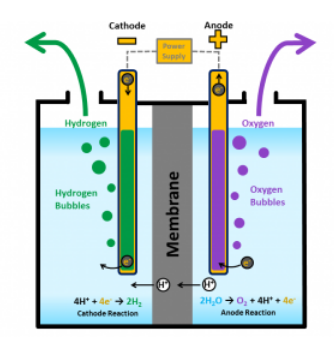
\includegraphics[width=0.4\linewidth]{figures/electrolysis.png}
	\hfill
	\caption{Production of hydrogen by electrolysis.}
	\label{fig:electro}
\end{figure}

Solid oxide electrolyzers must operate at thermperatures high enough for the solid oxide membranes to function properly (about 700$^{\circ}$-800$^{\circ}$C). The use of heat at these elevated temperatures decreases the amount of electrical energy needed to produce hydrogen from water.

\subsection{Iodine-Sulfur Thermochemical Cycle}

The concept of using nuclear heat as an energy source and water as a resource allows the possibility of much more sustainable industrial production without greenhouse gases. The most simple and promising methods, in terms of efficiency, operate at very high temperatures, typically above 900$^{\circ}$C. For example, sulfur-based cycles (Fig. \ref{fig:isulfur}) use a sulfuric acid dissociation reaction that only works above 870$^{\circ}$C and whose efficiency increases with temperature \cite{cea_gas-cooled_2006}. 

The NGNP aims to produce 500 kg/h of $H_2$ by using 50MWth. It will also produce hydrogen by high-temperature electrolysis with an equivalent output power of 5MWth and 20MWe.

\begin{figure}[H]
	\centering
	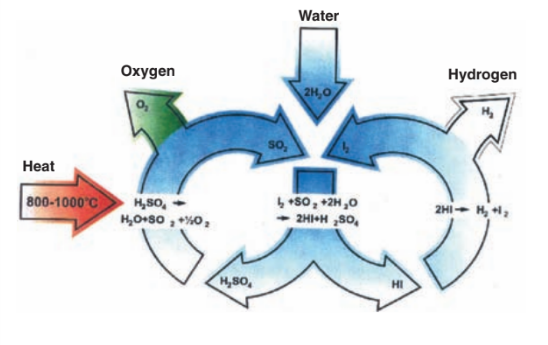
\includegraphics[width=0.4\linewidth]{figures/iodine-sulfur.png}
	\hfill
	\caption{Production of hydrogen by iodine-sulfur themochemical cycle.}
	\label{fig:isulfur}
\end{figure}

\section{HTGR Process Heat Application}

One of R&D projects for the high tmeperature gas-cooled reactor is to develop more efficient energy conversion cyclse. The gas turbine/steam turbine (GS-ST) combined cycle is a practicable approach to imporve the HTGR energy conversion efficiency.

The HTR-10 design features allow it to accept a gas/gas intermediate heat exchanger in series with the steam generator, which gives the HTR-10 flexibility for multi-aspect applications. Fig. \ref{fig:gtst} shows the conceptual flow scheme of the GT-ST combined cycle for the HTR-10.

With adoption of the IHX and double cycles, the economic competitiveness is decreased and the system operation and control are more complex.

\cite{yuanhui_htgr_1996}

\begin{figure}[H]
	\centering
	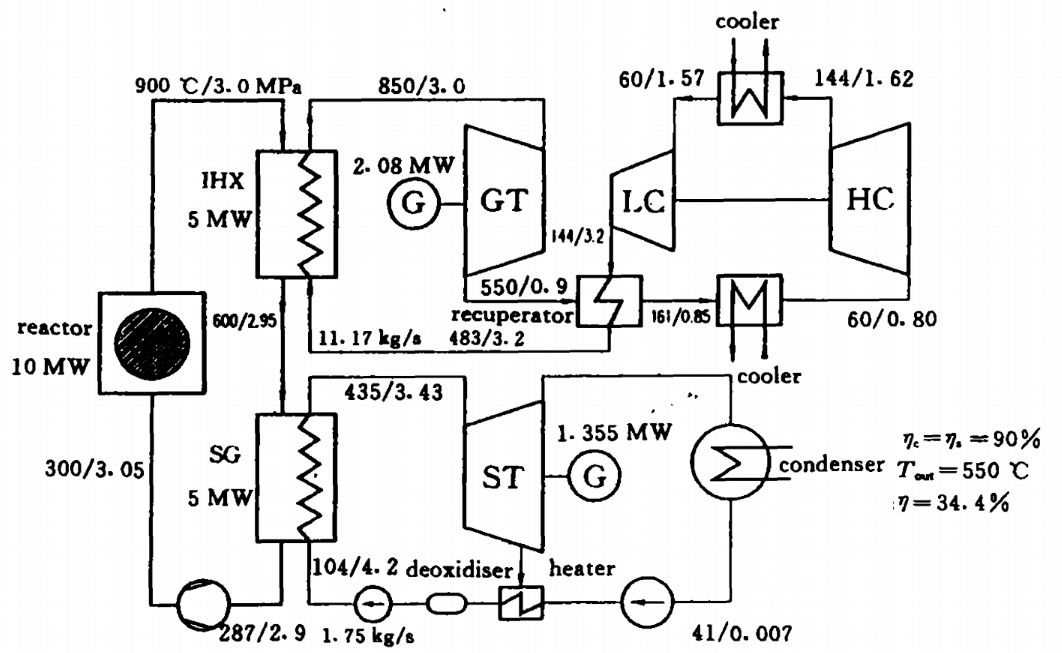
\includegraphics[width=0.4\linewidth]{figures/htgr-gtst.png}
	\hfill
	\caption{Gas Turbine/Steam Turbine (GT-ST) combined cycle in HTR-10.}
	\label{fig:gtst}
\end{figure}

\pagebreak
\bibliographystyle{plain}
\bibliography{bibliography}

\end{document}
